\documentclass[10pt]{article}

\usepackage{graphicx}
\usepackage{amsmath,amsfonts,amssymb}

% use different colors for links:
\usepackage{color}
\definecolor{darkgreen}{rgb}{0.1,0.5,0.1}
\definecolor{darkblue}{rgb}{0.2,0.2,1.0}
\usepackage[colorlinks=true,linkcolor=darkblue,citecolor=darkblue,
            filecolor=darkblue,urlcolor=darkgreen]{hyperref}


\setlength{\textwidth}{6.2in}
\setlength{\oddsidemargin}{0.3in}
\setlength{\evensidemargin}{0in}
\setlength{\textheight}{8.9in}
\setlength{\voffset}{-1in}
\setlength{\headsep}{26pt}
\setlength{\parindent}{0pt}
\setlength{\parskip}{5pt}



% a few handy macros

\newcommand\matlab{{\sc matlab}}
\newcommand{\goto}{\rightarrow}
\newcommand{\bigo}{{\mathcal O}}
\newcommand{\half}{\frac{1}{2}}
%\newcommand\implies{\quad\Longrightarrow\quad}
\newcommand\reals{{{\rm l} \kern -.15em {\rm R} }}
\newcommand\complex{{\raisebox{.043ex}{\rule{0.07em}{1.56ex}} \hskip -.35em {\rm C}}}


% macros for matrices/vectors:

% matrix environment for vectors or matrices where elements are centered
\newenvironment{mat}{\left[\begin{array}{ccccccccccccccc}}{\end{array}\right]}
\newcommand\bcm{\begin{mat}}
\newcommand\ecm{\end{mat}}

% matrix environment for vectors or matrices where elements are right justifvied
\newenvironment{rmat}{\left[\begin{array}{rrrrrrrrrrrrr}}{\end{array}\right]}
\newcommand\brm{\begin{rmat}}
\newcommand\erm{\end{rmat}}

% for left brace and a set of choices
\newenvironment{choices}{\left\{ \begin{array}{ll}}{\end{array}\right.}
\newcommand\when{&\text{if~}}
\newcommand\otherwise{&\text{otherwise}}
% sample usage:
%  \delta_{ij} = \begin{choices} 1 \when i=j, \\ 0 \otherwise \end{choices}


% for labeling and referencing equations:
\newcommand{\eql}{\begin{equation}\label}
\newcommand{\eqn}[1]{(\ref{#1})}
% can then do
%  \eql{eqnlabel}
%  ...
%  \end{equation}
% and refer to it as equation \eqn{eqnlabel}.  


% some useful macros for finite difference methods:
\newcommand\unp{U^{n+1}}
\newcommand\unm{U^{n-1}}

% for chemical reactions:
\newcommand{\react}[1]{\stackrel{K_{#1}}{\rightarrow}}
\newcommand{\reactb}[2]{\stackrel{K_{#1}}{~\stackrel{\rightleftharpoons}
   {\scriptstyle K_{#2}}}~}

% Parts:

% set enumerate to give parts a, b, c, ...  rather than numbers 1, 2, 3...
\renewcommand{\theenumi}{\alph{enumi}}
\renewcommand{\labelenumi}{(\theenumi)}

% set second level enumerate to give parts i, ii, iii, iv, etc.
\renewcommand{\theenumii}{\roman{enumii}}
\renewcommand{\labelenumii}{(\theenumii)}

  % input some useful macros

\newcommand{\bv}{\bar v}


\begin{document}

% header:
\hfill\vbox{\hbox{AMath 586 / ATM 581}
\hbox{Homework \#5}\hbox{Due Thursday, June 13, 2019}}

{\bf Name:} Your name here
\vskip 5pt

Due to Canvas by 11:00pm PDT on the due date.

To submit, see \url{https://canvas.uw.edu/courses/1271892/assignments/4836612}

This extra credit set of problems is worth an additional 20 points.


These problems concern the propagation of waves in ``excitable media'', in
particular biological tissue, such as nerve axons or the heart wall, that
conduct electrical signals such as nerve pulses.  These tissues are
generally semi-permeable to certain ions (in particular calcium Na$^+$ and
potassium K$^+$) with a permeability that depends on the voltage jump across
the membrane.  The potential difference across the membrane also serves as a
driving force for the flow of ions through the open channels.  You don't
need to understand the biochemistry to do this project, but if you're interested
you can find more links (and figures, animations, etc.) at, e.g.
\begin{itemize}
\item \url{http://www.scholarpedia.org/article/FitzHugh-Nagumo_model}
\item \url{https://en.wikipedia.org/wiki/Hodgkin-Huxley_model}
\end{itemize}

The starting point is a simple system of two ODEs, the spatially-homogeneous
FitzHugh-Nagumo
equations, which have various forms in the literature.  We will use the form
\begin{equation}\label{FHNode}
\begin{split}
v'(t) &= \frac 1 \epsilon (g(v(t)) - w(t) + I_a),\\
w'(t) &= \beta v(t) - \gamma w(t).
\end{split}
\end{equation} 
For the function $g(v)$ we will again use the cubic function
\begin{equation}\label{fv}
g(v) = v(\alpha - v)(v-1).
\end{equation} 
The  numbers $\alpha,~\beta,~\gamma~,\epsilon$ and $I_a$ are parameters.

This is a simple model that exhibits many features of excitable media, and
is a simplification of the famous {\it Hodgkin-Huxley equations} that are a 
better model for nerve propagation.  In the FitzHugh-Nagumo equations 
$v(t)$ models the membrane potential while $w(t)$ models the concentration
of an ion.

This system of ODEs does not model wave propagation --- for that we need a
PDE in space and time (with one space dimension for propagation along a
nerve axon or two space dimension for a wave propagating on the surface of the
heart, say).  This will be done below (in 1 space dimension).

The ODE models a situation in which electric charge can flow
infinitely quickly through the fluid on either side of the membrane, so that
the potential jump across the membrane is the same at every point in space
and the PDEs reduce to an ODE in time.  

With the parameter values
\begin{equation}\label{parm1}
\alpha=0.3,\quad \beta = 1,\quad \gamma = 1,\quad I_a=0,\quad \epsilon =
0.001
\end{equation}
and initial data
\begin{equation}\label{ic1}
v(0) = v_0,\quad w(0)=0,
\end{equation} 
the solution to the ODEs \eqn{FHNode} exhibit two different sorts of
behavior, as shown in the figures below:

\hfil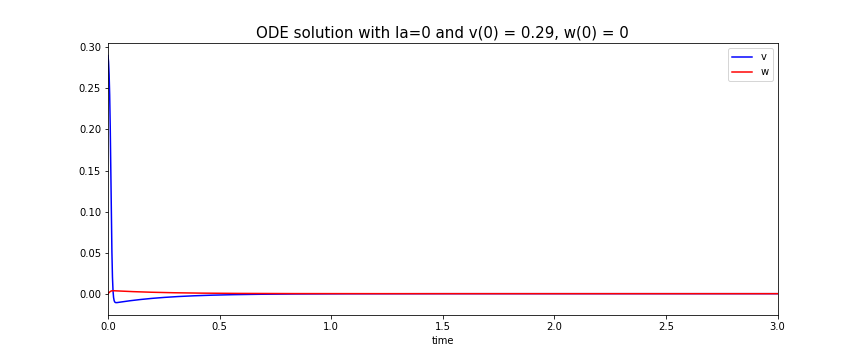
\includegraphics[width=5.0in]{v029.png}\hfil
\vskip 5pt
\hfil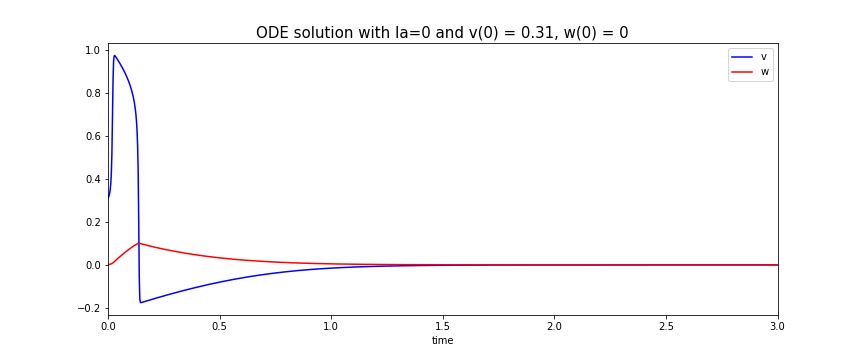
\includegraphics[width=5.0in]{v031.png}\hfil

\vskip 5pt

If $v_0=0.29$ then the initial membrane potential simply decays as ions flow
across the membrane and the solution approaches the stable steady state
$v=w=0$.

If $v_0=0.31$ then the initial membrane potential rises sharply to nearly
$v=1$, stays quite high for a bit, and then drops sharply and ultimately
decays back to the steady state.  This happens whenever $v_0$ is above the
``threshold value'' $\alpha = 0.3$.  This spike in potential is an ``action
potential'' in the language of neurophysiology, and in nerve cells the
propagation of action potential as waves is the manner in which nerve cells
communicate with one another.

The parameter $I_a$ is an applied current, a forcing term that can lead to
sustained oscillations (a train of nerve impulses in a nerve axon, for
example, once we add spatial variations).  
With the above parameter values and $v_0=0,~I_a=0.2$, the solution to
the ODE \eqn{FHNode} looks like:

\vskip 5pt
\hfil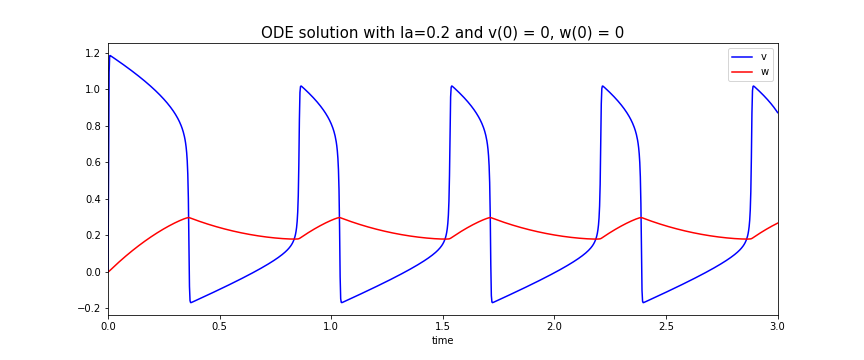
\includegraphics[width=5.0in]{Ia2.png}\hfil
\vskip 5pt

After the first action potential it settles down into a periodic
solution as the nerve ``fires'' repeatedly.

\newpage

To get some feel for what's going on, note that when $\epsilon$ is very small
we expect $v'(t)$ to be very large unless $w \approx g(v) + I_a$.  If we 
plot this cubic in the $v$--$w$ plane (the ``phase plane'') along with 
trajectories of the solution $(v(t), w(t))$, we get a plot like this, in
the case of repetitive firing:

\vskip 5pt
\hfil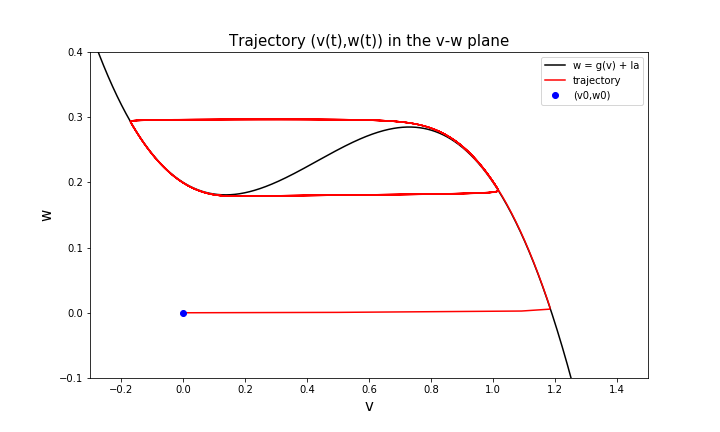
\includegraphics[width=4.5in]{FHtrajectory.png}\hfil
\vskip 5pt

Initially $v(t)$ changes very rapidly (with $w(t)\approx 0$) until it
hits the cubic. Then
the solution moves slowly along the cubic until it hits an extreme point 
after which $v$ adjusts very quickly (the nearly horizontal lines in the
trajectories) to reach a different part of the cubic, and then it varies
slowly again for a while. In the case shown it ultimately cycles around
the upper loop forever, once for each action potential.
Some other plots with more information are
shown at \url{http://www.scholarpedia.org/article/FitzHugh-Nagumo_model}.



\vskip 10pt
{\large\bf Problem 7.} 
\vskip 10pt
\begin{enumerate} 
\item Write a code using e.g. {\tt scipy.integrate.odeint} to solve
\eqn{FHNode} and reproduce the figures shown above as a test that it is working.  


\item Modify your code to also produce a phase plane plot similar to the plot
above.  Do this for each set of parameters used above, i.e. for
\[
\begin{split}
&I_a = 0, \quad v_0 = 0.29,\\
&I_a = 0, \quad v_0 = 0.31,\\
&I_a = 0.2, \quad v_0 = 0.
\end{split} 
\]

\item Experiment with varying $\epsilon$ and comment on what you observe,
both in terms of how the solution behaves (as a function of $t$ and in the
phase plane) and in terms of the computational method.
\end{enumerate} 

\vskip 10pt

{\bf The reaction-diffusion equations.}
In reality the charge doesn't
equilibrate infinitely quickly, but instead diffuses, and so we will add a
diffusion term to the equation for $v(t)$ to recover the PDEs.
In one space dimension:
\begin{equation}\label{FHN1d}
\begin{split}
v_t(x,t) &= v_{xx}(x,t) + \frac 1 \epsilon (g(v(x,t)) - w(x,t) + I_a(x)),\\
w_t(x,t) &= \beta v(x,t) - \gamma w(x,t).
\end{split}
\end{equation} 

Equation \eqn{FHN1d} is a reaction-diffusion equation.  Note that only $v$
diffuses but since $w_t$ depends on $v$ the solution will also show spatial
variations in $w$.

\vskip 10pt
{\large\bf Problem 8.} \vskip 10pt
\vskip 10pt

Create a notebook to solve the one-dimensional FitzHugh-Nagumo
equations \eqn{FHN1d}. You can base your code
on what you did for Allen-Cahn.   You will have to keep track of $w$ as well as
$v$ and modify the reaction terms for the FitzHugh-Nagumo reactions.
Again use the backward Euler method for these terms.  This will now require
solving a system of 2 equations for $V_j^{n+1}$ and $W_j^{n+1}$ at every
grid point.  Note, however, that the equation for $w$ is linear and so it is
possible to express $W_j^{n+1}$ as a function of $V_j^{n+1}$.  You
can use this to reduce the problem to a scalar cubic equation to
be solved for $V_j^{n+1}$, which can speed up the solution, or you
can simply use {\tt fsolve} on the system of two equations.


Test your code with the following two tests (feel free to experiment with
more):
\begin{enumerate}
\item
Use $m=499$ interior points on $-5\leq x\leq 5$ with parameter values
\begin{equation}\label{parm2}
\alpha=0.3,\quad \beta = 1,\quad \gamma = 1,\quad \kappa=0.2,\quad \epsilon =
0.001
\end{equation}
with no applied current ($I_a(x) = 0$) and initial data
\[
v(x,0) = \begin{choices} 1 \when |x|<1 \\  0 \when |x|>1 \end{choices}, \qquad
w(x,0) = 0.
\]
If you solve this out to time $t=1$, say, you should see a traveling wave 
develop and propagate.  Experiment with what size time step is needed and
discuss.

\item
Same situation as in part (a) but with initial data $v(x,0)=w(x,0)=0$ and
a spatially-varying applied current $I_a(x) = 0.8\exp(-5x^2)$.  
This models a situation in
which a stimulated nerve cell sends out a train of pulses.  Run the
computation out to time $t=2$ and you should see several pulses generated,
similar to the animation shown
\href{http://staff.washington.edu/rjl/classes/am586s2019/_static/FNmovie.html}{here} 
(on the class webpage for the final).  
This was generated using $m=499$ interior points and 1000 time steps. 

With coarser grids or larger timesteps you may get very poor solutions.
Experiment a bit and comment on your observations.


\end{enumerate} 


\end{document}
